% Sistema cartesiano con vectores base ê_1, ê_2, ê_3 (libro fig. 1.1)
\documentclass[border=4pt]{standalone}
\usepackage{tikz}
\usetikzlibrary{arrows.meta}
\begin{document}
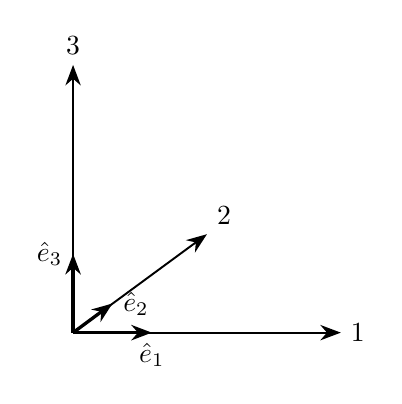
\begin{tikzpicture}[>={Stealth[length=2.6mm]}, line width=0.7pt]
  % ejes
  \draw[->] (0,0)--(3.4,0) node[right]{$1$};
  \draw[->] (0,0)--(1.7,1.25) node[above right]{$2$};
  \draw[->] (0,0)--(0,3.4) node[above]{$3$};
  % vectores base unitarios (cortos, gruesos)
  \draw[->, line width=1.2pt] (0,0)--(1.0,0) node[below]{$\hat e_1$};
  \draw[->, line width=1.2pt] (0,0)--(0.5,0.37) node[right]{$\hat e_2$};
  \draw[->, line width=1.2pt] (0,0)--(0,1.0) node[left]{$\hat e_3$};
\end{tikzpicture}
\end{document}
